% !TEX root = paperVersion2.tex
\documentclass[conference]{IEEEtran}
\IEEEoverridecommandlockouts

% ── IEEE-standard font: Times New Roman via fontspec (XeTeX/LuaTeX) ───────────
\usepackage{fontspec}
\setmainfont[Ligatures=TeX]{Times New Roman}
\setsansfont[Ligatures=TeX]{Arial}
\setmonofont{Courier New}

% ── Packages ─────────────────────────────────────────────────────────────────
\usepackage{cite}
\usepackage{amsmath,amssymb,amsfonts}
\usepackage{graphicx}
\usepackage{textcomp}
\usepackage{xcolor}
\usepackage{booktabs}
\usepackage{multirow}
\usepackage{url}
\usepackage{microtype}
\usepackage{array}

% Figures live in two folders: the notebook's persisted images and the legacy set.
\graphicspath{{assignment2_baseline/images/}{figures/}}

% ═════════════════════════════════════════════════════════════════════════════
%  paperVersion2.tex — extended study (classical + deep learning + MARBERT/LoRA)
%  All result numbers are taken from results/all_model_metrics.json (22 models).
%  Figures are auto-persisted by the notebook to assignment2_baseline/images/.
% ═════════════════════════════════════════════════════════════════════════════

\begin{document}

% ── Title & Author ────────────────────────────────────────────────────────────
\title{From Bag-of-Words to Parameter-Efficient Transformers:\\
A Controlled Comparison of 22 Models for Arabic\\
Sentiment Analysis on the ASTD Corpus}

\author{
  \IEEEauthorblockN{Rayyan Tawfieg}
  \IEEEauthorblockA{
    \textit{Department of Electrical and Computer Engineering}\\
    \textit{Birzeit University}\\
    West Bank, Palestine\\
    rayyantawfieg@gmail.com
  }
}

\maketitle

% ── Abstract ─────────────────────────────────────────────────────────────────
\begin{abstract}
Arabic sentiment analysis has proven to be difficult, due to its rich number of
dialect variations, limited dataset and corpus availability, complex term
morphology, and imbalanced datasets. In our dataset, the Arabic Sentiment Tweets
Dataset (ASTD), about three quarters of the tweets fall under the neutral or
objective class. If we were to build a model that always predicts the majority
class, we would achieve an accuracy of around 75\% which is a misleading metric
to accept as appropriate here. Earlier studies barely compared the results of
classical, deep-learning, and transformer methods in one place, especially with
metrics this intricate. We present a comparison of 20+ models trained on the ASTD
with a fixed 60/20/20 split, seed, and primary metric (macro F1), on a low-resource
computing environment with no CUDA or half-precision and limited memory of 16~GB.
We included transformers such as MARBERT and implemented low-rank adaptation, which
helped us reduce the trained parameters from its monstrous 163M to merely less than 1\% of that,
which actually ended up being the best-performing model of them all, achieving a macro F1
score of 65\% versus the classical or conventional counterparts, which scored around 50\%
(a stemmed linear SVM), as well as a big jump over the vanilla CNN architecture that achieved
46\% macro F1. We found that regularisation techniques proved to be beneficial in our results;
label smoothing and stemming were the main contributors, while focal loss, which we only
tested jointly with a higher LoRA rank and augmentation, did not outperform label smoothing.
When using the transformer, we found a major jump in costs: memory usage jumped 2700$\times$
with far higher latency than the SVM model we built. These trade-offs are important for
anyone who wants to use these models in production, where computing resources are costly. We
go over every model's performance and cost in detail throughout the paper in both figures and statistics.
\end{abstract}

% ── I. Introduction ───────────────────────────────────────────────────────────
\section{Introduction}

Sentiment analysis is the process of reading an input of text and making a
decision on whether the text expresses a positive, negative, neutral, or objective
point. This is easier in English, where the morphology is simpler and the language
is more widely used worldwide, especially on social media. Arabic, however,
is not that simple. It remains difficult for three main reasons.

\textbf{Morphology.} 
Arabic terms are structured from a three-letter base; from there, using morphology
via prefixes, suffixes, or even vowel pronunciation changes, we create many variations
of the same word. So if we were to use a counting-based model, we would treat each variation
as an individual word instead of part of the original, causing individual words to be rare in
count while the number of distinct word forms increases heavily --- a sparsity that
is a direct result from Arabic's complex morphology~\cite{antoun2020arabert}.

\textbf{Dialect.}
Standard Arabic is the formal register worldwide, but on social media people can
customise and write in their own dialect, which could be Egyptian, Palestinian, Moroccan,
Jordanian, Saudi Arabian, etc. Each differs greatly in what words mean and how they are spelled;
for example, لبن (Laban) means milk in Egyptian, but in Levantine it means yogurt. Even human
speakers show uneven mutual intelligibility across dialects --- Moroccan Arabic, for instance,
is notably difficult for a Levantine speaker to understand~\cite{zaidan2014dialect} --- so a
model trained on one dialect's data cannot be assumed to generalise to another.

\textbf{Data.} 
Due to Arabic being a minority language, labelled Arabic sentiment datasets are rare, small, and imbalanced.
The Arabic Sentiment Tweets Dataset (ASTD)~\cite{nabil2015astd}, our test set, is small and imbalanced, having
just under ten thousand tweets, each labelled as either negative, positive, objective, or neutral.
The imbalance comes from the fact that the objective/neutral class accounts for nearly three quarters of the dataset.
Therefore, if a model were to only select the majority class, it would score an accuracy of 75\% which is misleading.
Thus, we use macro F1 as our primary metric, as it is a better metric for imbalanced datasets.

Previous research on the ASTD dataset has been limited: it was done either with classical methods~\cite{nabil2015astd}
or, more recently, transformer-based models~\cite{antoun2020arabert,abdulmageed2021marbert}, but rarely are all methods
found together in one place and trained under the same conditions. To push things even further, we also
account for cost in terms of memory, latency, training time, and inference time, monitored throughout all the models.
These metrics help us infer how much improvements actually cost us over the previous generation of models.

Our work here is designed to close this gap, with precise control over the experiments,
while training a multitude of models of various architectures and reporting their performance and cost.
Every experimental model holds the dataset split, the seed, and the metric constant. This way the differences are
limited to the variable under test and not the other factors. Our contributions are:

\begin{itemize}
  \item A \textbf{fair comparison among 22 models} spanning classical, deep-learning,
        and transformer architectures, and variants of each, all trained with the same data
        and environment and evaluated equally on the same metrics.
  \item An analysis of \textbf{reduced parameter training}: training MARBERT with LoRA
        trains only under a single percent of the parameters, yet achieves the highest macro F1.
        This is crucial for low-resource training, saving computation and memory, and
        enabling us to develop this model on a 16~GB device.
  \item A \textbf{study of the skewed label distribution solutions}: we implemented four individual
        approaches to the skewed schema dominated by the objective class: merging it with
        the neutral class, dropping it, keeping the dataset in its vanilla state, or downsampling the
        class to match the other minorities. All were then evaluated on which schema yielded the best results.
  \item A study of \textbf{imbalance-handling methods}: inverse-frequency class weights
        were applied as a constant baseline across every model, on top of which we
        isolated four further interventions : label smoothing, SMOTE, back-translation,
        and downsampling. In addition we added one combined configuration adding focal loss alongside
        a higher LoRA rank and augmentation, to indicate which actually helps.
  \item A detailed \textbf{accuracy vs.\ efficiency} analysis, numerically expressing
        the trade-offs of using a lightweight traditional model versus a denser deep-learning model
        on low-resource hardware. 
\end{itemize}


This scope is broken down in to four research inqueries (RQ1--RQ4), detailed in 
Section~III. The remainder of this paper covers the related work (Section~II);
the model design and methodology (Sections~III--VI); the result analysis (Sections~VII--VIII); and a discussion
of trade-offs, limitations, and conclusions (Sections~IX--X).


% ── II. Related Work ──────────────────────────────────────────────────────────
\section{Related Work}

\subsection{Historic Machine Learning}
The pioneering Arabic sentiment systems were traditional classifiers; the idea was
simple in terms of today's architectures: they turned each record into a ``bag of words'' and
trained the model on it. Rushdi-Saleh et~al.\ built the corpus for Arabic and concluded that SVMs
exceed Naive Bayes in performance~\cite{rushdi2011oca}. Abdul-Mageed and Diab's AWATIF
built a multi-genre MSA corpus annotated for subjectivity and sentiment, showing that
linguistically-motivated, genre-aware annotation guidelines yield substantially higher
inter-annotator agreement than simple guidelines~\cite{abdulmageed2012awatif}.
Nabil et~al.\ released ASTD and showed that classifiers score far higher weighted accuracy
on the unbalanced split than the balanced one~\cite{nabil2015astd} --- exactly the kind of
majority-class-inflated metric that motivates our use of macro F1, and in essence the issue
we are trying to research here. SVMs remain a strong text-classification baseline, as does
random forest.

\subsection{Word Embeddings \& Data Representations}
Word2Vec learns words as vectors and bundles together vectors that appear in similar contexts,
which leads them to have similar representations. FastText is the next level of
that, where we use the n-gram methodology: we break a word into subwords, which is great for languages
that have morphological structure in their vocabulary. This is subsequently great for Arabic,
because even so-called ``new words'' would not be considered new anymore, since their subwords are
shared with other words from the same source. Arabic-tailored
vectors have been shown to give an upper hand over generic multilingual ones when applied to Arabic.
The limiting factor is that mean-pooling a tweet is not order-oriented, so phrases like
``I do not like this'' and ``I like this'' turn into nearly identical vectors.

\subsection{Deep Learning}
Kim illustrated that a CNN model proved to be quite an improvement in performance for
short-text classification~\cite{kim2014cnn}. RNN and LSTM architectures
read text sequentially while maintaining context to some extent. However, since tweets tend to be short,
this context was proven to provide only a limited benefit to the classifier.

\subsection{Arabic Language Transformers}
The transformer and BERT redirected NLP approaches. A more tailored approach was AraBERT, which retrained
BERT on roughly 24~GB (70 million sentences) of Arabic text~\cite{antoun2020arabert}. As extensive as that is,
MARBERT~\cite{abdulmageed2021marbert} is more relevant to our work, as it was
trained on over a billion Arabic tweets while taking dialect into consideration.
Given its extensive dataset and the familiar nature of its data, it was deemed the most natural
transformer to use for our task, as it has also been used in models implemented today.

\subsection{Fine Tuning Efficiency with Parameters}

Fine-tuning a 163M-parameter model is expensive, especially in memory and computation.
Adapter methods insert small trainable sections while freezing the foundation.
LoRA~\cite{hu2022lora}, which in a way works like dimensionality reduction, injects trainable low-rank
matrices, which helps reduce the number of trainable parameters to a fraction of a percent of the weights
while matching almost full fine-tuning on tasks, all while being feasible to train on lower-end hardware
such as a 16~GB laptop.

\subsection{Class Imbalance and Augmentation}
Dealing with imbalanced datasets is not a new field and has been studied for a
considerable amount of time. Many approaches have been proposed to deal with this issue,
such as making minority-class mistakes cost more
during training, or down-weighting the majority class (Focal Loss)~\cite{lin2017focal},
regularising confident predictions (Label Smoothing)~\cite{muller2019labelsmoothing},
increasing the minority class to help balance the dataset (SMOTE)~\cite{chawla2002smote},
generating synthetic Arabic sentences via round-trip translation (Arabic$\to$English$\to$Arabic)
through pretrained machine translation systems~\cite{tiedemann2020opusmt}, an adaptation of the
back-translation augmentation technique~\cite{sennrich2016backtranslation}.
All were evaluated individually and monitored closely.

\subsection{Summary and Gap}
Table~\ref{tab:related} shows a summary of previous work and how each prior study handled
each type individually, but none of them evaluated all of them together in a single, unified manner.
Add to that extensive cost monitoring, and that is what this paper does.

\begin{table}[h]
  \centering
  \caption{Coverage of Related Work on Arabic Sentiment Analysis}
  \label{tab:related}
  \setlength{\tabcolsep}{4pt}
  \begin{tabular}{lcccc}
    \toprule
    \textbf{Study} & \textbf{Classic} & \textbf{Deep} & \textbf{Transf.} & \textbf{ASTD} \\
    \midrule
    Rushdi-Saleh et al.~\cite{rushdi2011oca}          & \checkmark &            &            &            \\
    Abdul-Mageed \& Diab~\cite{abdulmageed2012awatif} & \checkmark &            &            &            \\
    Nabil et al.~\cite{nabil2015astd}                 & \checkmark &            &            & \checkmark \\
    Kim~\cite{kim2014cnn}                             &            & \checkmark &            &            \\
    Antoun et al.~\cite{antoun2020arabert}            &            &            & \checkmark &            \\
    Abdul-Mageed et al.~\cite{abdulmageed2021marbert} &            &            & \checkmark & \checkmark \\
    \textbf{This work}                                & \checkmark & \checkmark & \checkmark & \checkmark \\
    \bottomrule
  \end{tabular}
\end{table}

% ── III. Experimental Design ──────────────────────────────────────────────────
\section{Experimental Design}

This study focuses on four research questions (RQ1--RQ4) that are answered
by holding everything constant while tweaking a certain aspect of the process:
\begin{itemize}
  \item[\textbf{RQ1}] Does changing how the dominant objective class is handled change performance? 
  \item[\textbf{RQ2}] Against a constant class-weighted baseline, does data augmentation
  (SMOTE, back-translation) improve minority classification better than simpler
  techniques such as stemming or label smoothing?
  \item[\textbf{RQ3}] Does a pretrained transformer such as \textbf{MARBERT+LoRA}
  outperform classical and vanilla deep-learning models on the same resource budget?   
  \item[\textbf{RQ4}] Is \textbf{parameter-efficient LoRA} an effective way to
        train models with extensive parameters when constrained by a limited corpus and resources?
\end{itemize}

\subsection{Label Schemas}
The ASTD resource has a four-class distribution (positive, negative, objective, and neutral)
that can be handled with multiple approaches. In our study, instead of evaluating just one
schema, we evaluate four different schemas (Table~\ref{tab:schemas}). This way, we can later conclude
how each schema affects performance rather than assume it. And since each schema
can differ in test-set size and number of classes, using absolute macro F1 is not directly
comparable across all the schemas. We therefore read the schema results from how each model reacts
to the change.

\begin{table}[h]
  \centering
  \caption{The Four Label Schemas Evaluated}
  \label{tab:schemas}
  \setlength{\tabcolsep}{3.5pt}
  \begin{tabular}{llcc}
    \toprule
    \textbf{Schema} & \textbf{Definition} & \textbf{Classes} & \textbf{Test $N$} \\
    \midrule
    A & OBJ merged into NEUTRAL            & 3 & 1{,}939 \\
    B & OBJ dropped entirely              & 3 & 645     \\
    C & Original four-class               & 4 & 1{,}939 \\
    D & Four-class, OBJ downsampled to 1{,}500 & 4 & 945 \\
    \bottomrule
  \end{tabular}
\end{table}

\subsection{Protocol}
There is an understanding, or what others would call a convention, that was applied to all the models:
a stratified \textbf{60/20/20} train/validation/test split of the schema; a random state of 42
(which makes reproducing results possible even with ``randomness''); and \textbf{macro F1} as the primary
metric, since accuracy is misleading and does not express true performance when the dataset has a huge
majority for one class. Model hyperparameters are decided based on the output of the validation set. Finally,
all extractors and tokenizers are fit on the training set only.

\subsection{Metrics and Benchmarking Harness}
Once every model is trained, each is passed to a utility method that logs a selection
of metrics for each model, regardless of the framework. We monitor the following: accuracy, macro F1,
weighted F1, confusion matrix, parameter and trainable-parameter counts, layer count, size in memory,
training time, and inference time. This makes comparing models on both quality and cost possible.


% ── IV. Dataset and Preprocessing ─────────────────────────────────────────────
\section{Dataset and Preprocessing}

\subsection{The Dataset}
We used the ASTD~\cite{nabil2015astd}. It is composed of over 9,600 tweets,
labelled as positive, negative, neutral, and objective. Under the primary schema (A), we merged
the neutral and objective classes together. On inspection, we found 10 invalid rows, which were
dropped since they were now empty after preprocessing and removing stop words (words that do
not add value to a sentence). Table~\ref{tab:dist} and Fig.~\ref{fig:dist} express the
distribution of the dataset, showing how three quarters of the dataset is the newly merged
neutral class.

\begin{table}[h]
  \centering
  \caption{ASTD Class Distribution (Schema A, OBJ merged into NEUTRAL)}
  \label{tab:dist}
  \begin{tabular}{lrr}
    \toprule
    Class   & Count & Proportion \\
    \midrule
    NEUTRAL & 7,274 & 75.1\%     \\
    NEG     & 1,641 & 17.0\%     \\
    POS     &   769 &  7.9\%     \\
    \midrule
    Total   & 9,684 & 100\%      \\
    \bottomrule
  \end{tabular}
\end{table}

\begin{figure}[t]
  \centering
  
\includegraphics[width=\columnwidth]{class_distribution.png}
  \caption{ASTD class distribution. Three quarters of the corpus is neutral;
           positive tweets are the rarest at about 8\%. This imbalance is the
           central difficulty of the task.}
  \label{fig:dist}
\end{figure}

\subsection{Two Preprocessing Pipelines}
Two different preprocessing plans were executed, since the nature of the input for each model,
classical and transformer, varies.

\textbf{Classical pipeline} (TF-IDF, Word2Vec, FastText): 
This approach was aggressive; we removed things such as hashtag symbols, mentions, URLs, and
HTML content. We then normalised the Arabic words by reducing letter variants to
single forms. We also removed stop words, words that provide no sentiment value in a
sentence. 

\textbf{Transformer pipeline} (MARBERT): 
This approach was lighter: we only stripped URLs, mentions, and diacritics, and
normalised the letter variations. Stop words and punctuation were \emph{kept},
because the pretrained model already accounts for them and MARBERT consumes raw
WordPiece tokens. WordPiece is how MARBERT reads a word: it divides the word into
sub-word parts and marks any piece that continues the previous one with
\texttt{\#\#} --- for example, ``playing'' becomes \texttt{play} + \texttt{\#\#ing},
where \texttt{\#\#} signals that ``ing'' attaches to the ``play'' token.

% ── V. Methodology ────────────────────────────────────────────────────────────
\section{Methodology}

Fig.~\ref{fig:pipeline} helps summarise the following content as a pipeline-style informational
image.

\begin{figure*}[t]
  \centering
  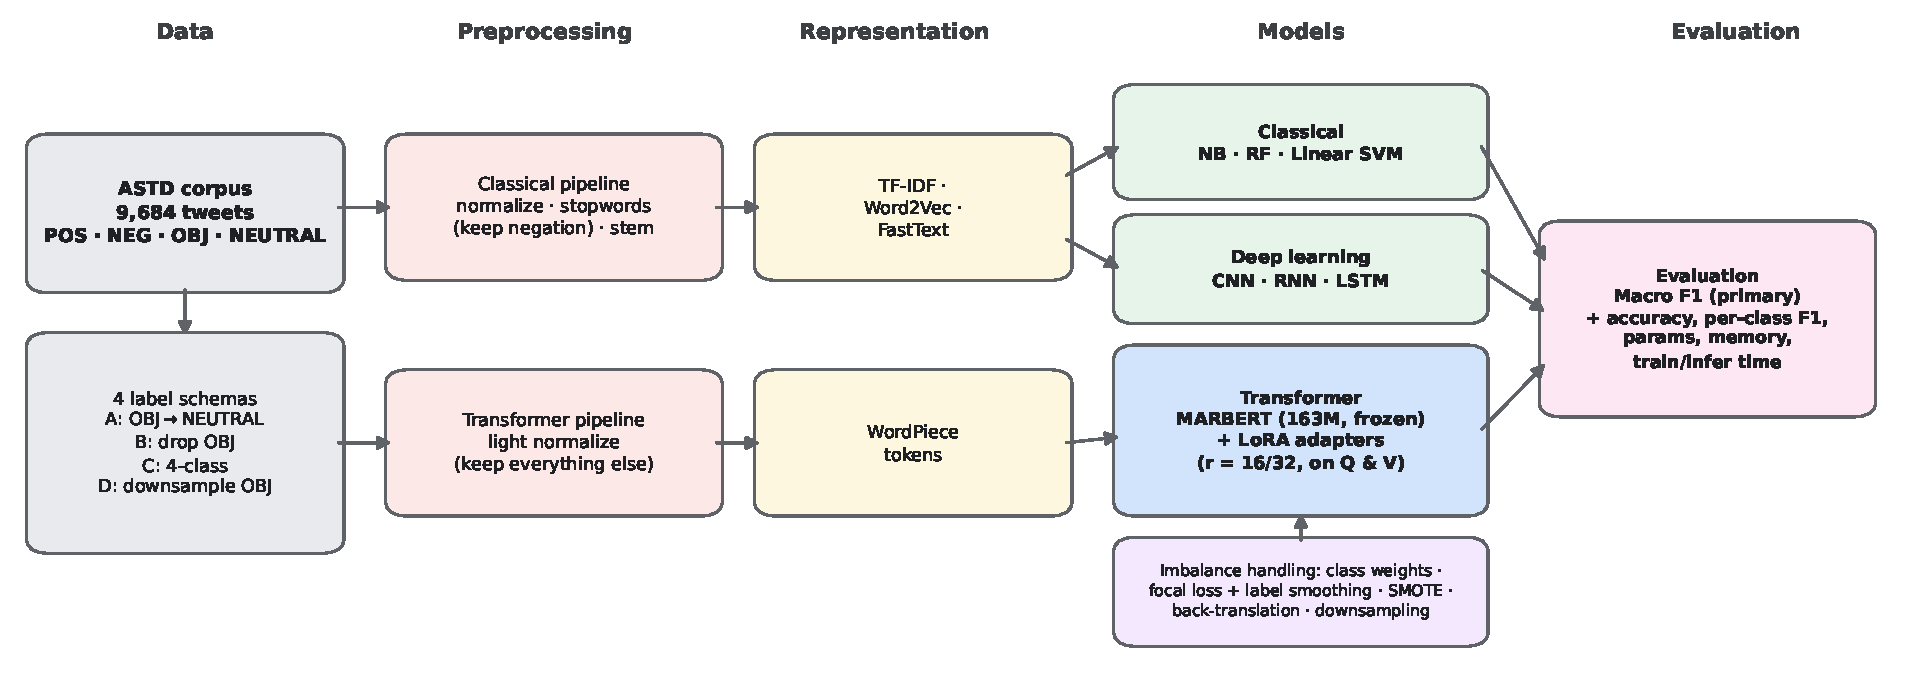
\includegraphics[width=\textwidth]{fig_pipeline.pdf}
  \caption{End-to-end experimental pipeline. The ASTD corpus is organised into
           four label schemas and passed through two preprocessing pipelines
           into three model families; the imbalance interventions feed model
           training, and every model is scored by one shared metric harness.
           The 60/20/20 split and seed~42 are held constant throughout.}
  \label{fig:pipeline}
\end{figure*}

\subsection{Feature Representations}
\textbf{TF-IDF} 
Term Frequency--Inverse Document Frequency, is the process of giving a term
a value based on the combination of how frequent it is in a document and how rare it is
among all the documents:
\begin{equation}
  \mathrm{TF\text{-}IDF}(t,d)
    = \bigl(1 + \log\,\mathrm{tf}(t,d)\bigr)\cdot
      \log\!\frac{N}{\mathrm{df}(t)+1}.
  \label{eq:tfidf}
\end{equation}

In this process we preserved the top 10,000 useful unigrams and bigrams (bigrams so that we
capture negating terms such as ``not like''), ignoring terms that only showed up in one document.
In contrast, for \textbf{Word2Vec} (100-d, CBOW) and \textbf{FastText} (300-d, sub-word),
a tweet is expressed via mean pooling (taking all words in a tweet and averaging them to represent
the whole tweet). FastText's sub-term structure enables dealing with unseen spellings.


\subsection{Classical Models}
\textbf{Na\"{i}ve Bayes} is a statistical classifier, built with TF-IDF only, as it
cannot take negative values as input, along with tuned smoothing $\alpha$ (which handles unseen
words so they do not get a probability of zero). \textbf{Random Forest} was trained
with all three data representations (RF + TF-IDF, RF + Word2Vec, RF + FastText), all
while tuning the tree count, the maximum depth of each tree, and the class balancing (which makes minorities
count more during tree building). \textbf{Linear SVM} was trained with
the same word-level TF-IDF representation as Na\"{i}ve Bayes and Random Forest, alongside
balanced classes, light stemming, and the two data-augmentation variants
of Section~\ref{sec:imbalance}.


\subsection{Deep Learning Models}
The three deep-learning architectures, CNN, RNN, and LSTM, share common ground. They are
all trainable, with a 100-dimension embedding over a 10,000-word vocabulary, all while
taking 50-token inputs (valid since tweets are around this size). The CNN takes advantage
of its structure, using width-3 kernels and max pooling. The RNN and LSTM models read sequentially. All the
deep-learning models adopted Adam (momentum + per-weight step) and early stopping. 

\subsection{Transformer: MARBERT + LoRA}
We used the MARBERT~\cite{abdulmageed2021marbert} transformer with LoRA~\cite{hu2022lora}.
The pretrained weights were conserved, while we only added a couple of rank-$r$ matrices,
$A$ and $B$, so that each adapted weight is calculated via:
\begin{equation}
  W = W_0 + \tfrac{\alpha}{r}\,BA, \qquad r \ll \min(d,k),
  \label{eq:lora}
\end{equation}
We ran a comparison of a pair of $r$ values, 16 and 32, where in both cases
we stay below training even 1\% of the original parameters. LoRA proved useful here,
since we cannot fully train and tune on a corpus this small (it would result in memorising
details and overfitting), and it keeps training feasible given our resource budget.

\subsection{Class-Imbalance Handling}
\label{sec:imbalance}
\textbf{(1) Inverse-frequency class weights} made it so that each error classifying the
positive and negative classes is penalised significantly more than errors on the majority class.
This was applied as a baseline for all models in the paper as well as SVM and Random Forest; four further
interventions were each tested in isolation against the plain weighted baseline:
\textbf{(2) label smoothing}~\cite{muller2019labelsmoothing} (0.05), which gives the
model a sense of doubt so it does not predict too confidently, in turn allowing it to generalise better;
\textbf{(3) SMOTE}~\cite{chawla2002smote}, a method of data augmentation where we take the gap between
two vectors in the same group and generate a new one in between, thus adding new data grouped
with the minority class; \textbf{(4) back-translation}, which takes our Arabic input, translates
it to English, then back to Arabic, generating new data that can be labelled instantly; and
\textbf{(5) downsampling}, a cruder way of handling things that can actually cause lower
performance, since we eliminate rows from the majority (objective) class --- this is Schema D.
Separately, we also trained one combined configuration adding \textbf{focal loss}~\cite{lin2017focal}
(which turns down the signal from easy majority-class examples so the model focuses on the harder
minority ones) alongside a higher LoRA rank and back-translation augmentation (Section~\ref{sec:rq2});
because all three changes were made at once, focal loss's contribution cannot be concluded on its own.


% ── VI. Experimental Setup ────────────────────────────────────────────────────
\section{Experimental Setup}

Table~\ref{tab:setup} expresses, in a brief and concise manner, the configuration that
was used across the experiments.

\begin{table}[t]
  \centering
  \caption{Experimental configuration.}
  \label{tab:setup}
  \setlength{\tabcolsep}{5pt}
  \begin{tabular}{ll}
    \toprule
    \textbf{Parameter} & \textbf{Value} \\
    \midrule
    \multicolumn{2}{l}{\textit{Data \& protocol}}\\
    Dataset             & ASTD, 9{,}684 tweets (after cleaning) \\
    Train / Val / Test  & 5{,}810 / 1{,}937 / 1{,}937 (60/20/20, stratified) \\
    Random seed         & 42 \\
    Primary metric      & Macro F1 \\
    \midrule
    \multicolumn{2}{l}{\textit{Classical (NB, RF, SVM)}}\\
    Features            & 10{,}000 word-level TF-IDF terms (1--2-grams) \\
    Hyper-parameters    & 3-fold \texttt{GridSearchCV} on macro F1 \\
    \midrule
    \multicolumn{2}{l}{\textit{Deep learning (CNN, RNN, LSTM)}}\\
    Embedding           & 100-d, trainable \\
    Max sequence length & 50 tokens \\
    Optimiser           & Adam \\
    Early stopping      & patience 5 (best val macro F1) \\
    \midrule
    \multicolumn{2}{l}{\textit{Transformer (MARBERT + LoRA)}}\\
    Optimiser           & AdamW \\
    Learning rate       & $1$--$2\times10^{-4}$, 10\% warmup \\
    Weight decay        & 0.01 \\
    Batch size          & 16 \\
    Epochs              & up to 6 (best val macro F1) \\
    Max sequence length & 128 tokens \\
    LoRA rank $r$       & 16 and 32 \\
    LoRA $\alpha$ / dropout & $2r$ / 0.05 \\
    LoRA target modules & query, value \\
    \midrule
    \multicolumn{2}{l}{\textit{Hardware \& software}}\\
    Hardware            & Apple M1~Pro, 16~GB unified memory \\
    Backend             & Metal (MPS); no CUDA, no fp16 \\
    Frameworks          & PyTorch + HF Transformers/PEFT; \\
                        & TensorFlow/Keras; scikit-learn/Gensim \\
    Python              & 3.12 \\
    \bottomrule
  \end{tabular}
\end{table}

\textbf{Why use macro F1?} It averages the F1 while taking the weight of each class
into consideration, so a model that ignores the minority classes performs poorly regardless of its overall
accuracy.
% ── VII. Results ──────────────────────────────────────────────────────────────
\section{Results}

\subsection{Overall Comparison}
We created two tables to help express the results: Table~\ref{tab:perf} expresses
the overall performance of the 22 models, and Table~\ref{tab:cost} illustrates what
each configuration cost to train. We do not illustrate the schema models here, since
their architecture is the same, so they share their family's cost. The four subsections
below answer RQ1--RQ4 in turn.

\begin{table}[t]
  \centering
  \caption{Test Performance for All 22 Configurations (Primary Metric: Macro F1).
           Best per family in \textbf{bold}; overall best among the primary-schema
           rows (top four blocks, shared $N{=}1{,}937$ test set) \underline{underlined}.
           The schema-ablation blocks (bottom two) use different test-set sizes
           (Table~\ref{tab:schemas}) and are excluded from the overall-best comparison
           --- see \S\ref{sec:rq1}.}
  \label{tab:perf}
  \setlength{\tabcolsep}{3.5pt}
  \begin{tabular}{llccc}
    \toprule
    \textbf{Model / Config} & \textbf{Cls} & \textbf{Acc} & \textbf{Macro F1} & \textbf{Wtd F1} \\
    \midrule
    \multicolumn{5}{l}{\textit{Classical (Schema A, 3-class)}}\\
    Na\"{i}ve Bayes + TF-IDF    & 3 & 0.741 & 0.424 & 0.693 \\
    Random Forest + TF-IDF      & 3 & 0.736 & 0.380 & 0.674 \\
    Random Forest + Word2Vec    & 3 & 0.683 & 0.403 & 0.661 \\
    Random Forest + FastText    & 3 & 0.687 & \textbf{0.431} & 0.673 \\
    \midrule
    \multicolumn{5}{l}{\textit{Deep learning (3-class)}}\\
    CNN                         & 3 & 0.598 & \textbf{0.455} & 0.626 \\
    RNN                         & 3 & 0.531 & 0.374 & 0.581 \\
    LSTM                        & 3 & 0.594 & 0.448 & 0.623 \\
    \midrule
    \multicolumn{5}{l}{\textit{Linear SVM (3-class)}}\\
    SVM + TF-IDF                & 3 & 0.695 & 0.481 & 0.690 \\
    SVM + Stemmed TF-IDF        & 3 & 0.708 & \textbf{0.507} & 0.702 \\
    SVM + Back-Translation      & 3 & 0.708 & 0.483 & 0.696 \\
    SVM + SMOTE                 & 3 & 0.641 & 0.451 & 0.651 \\
    \midrule
    \multicolumn{5}{l}{\textit{Transformer: MARBERT + LoRA (3-class)}}\\
    MARBERT LoRA $r{=}16$       & 3 & 0.717 & 0.626 & 0.736 \\
    MARBERT LoRA $r{=}16$ + LS  & 3 & 0.740 & \underline{\textbf{0.650}} & 0.757 \\
    MARBERT LoRA $r{=}32$ + Aug & 3 & 0.693 & 0.616 & 0.716 \\
    \midrule
    \multicolumn{5}{l}{\textit{Label-schema ablation --- SVM (see \S\ref{sec:rq1})}}\\
    SVM Schema A (merged)       & 3 & 0.713 & 0.484 & 0.699 \\
    SVM Schema B (pure)         & 3 & 0.527 & 0.476 & 0.515 \\
    SVM Schema C (4-class)      & 4 & 0.644 & 0.410 & 0.631 \\
    SVM Schema D (downsampled)  & 4 & 0.500 & 0.463 & 0.495 \\
    \midrule
    \multicolumn{5}{l}{\textit{Label-schema ablation --- MARBERT}}\\
    MARBERT Schema A (merged)   & 3 & 0.686 & 0.621 & 0.710 \\
    MARBERT Schema B (pure)     & 3 & 0.670 & \textbf{0.669} & 0.677 \\
    MARBERT Schema C (4-class)  & 4 & 0.603 & 0.531 & 0.633 \\
    MARBERT Schema D (downsamp.)& 4 & 0.631 & 0.618 & 0.636 \\
    \bottomrule
  \end{tabular}
\end{table}

\subsection{RQ1: Does the Label Schema Matter?}
\label{sec:rq1}
Certainly, if we look at Fig.~\ref{fig:schemas} as well as each model:
the \textbf{four-class formulation (Schema C) is the least performant} for both SVM and
MARBERT. \textbf{Downsampling the majority (Schema D)} performs better than that, boosting macro F1 for
the SVM by around 5\% ($0.410\!\to\!0.463$) and for MARBERT by approximately 9\% ($0.531\!\to\!0.618$).
This confirms that having four classes is not the issue, but rather having a class that dominates the
dataset.

When we look at the \textbf{three-class schemas}, the SVM performs marginally better when the neutral
and objective classes are merged rather than dropped, scoring 48.4\% when merging and 47.6\% when
dropping --- a gap of under one point, which given our single-seed setup is not a meaningful
difference. The MARBERT architecture, on the other hand, favours dropping the objective class
entirely, which achieved the highest possible F1 at around 67\% (\textbf{0.669}) --- the highest raw
score in Table~\ref{tab:perf}, though it is not the table's underlined overall-best, since Schema B
uses a smaller, cleaner test set ($N{=}645$ vs.\ $N{=}1{,}937$) that is not directly comparable to
the other rows. Because Schema B uses a cleaner and smaller test set, we take this as evidence that
MARBERT separates pure sentiment classes very well once the ambiguous tweets are removed.

\begin{figure*}[t]
  \centering
  
\includegraphics[width=0.48\textwidth]{sec15_svm_schemas.png}
  \hfill
  
\includegraphics[width=0.48\textwidth]{sec15_marbert_schemas.png}
  \caption{Schema comparison for SVM (left) and MARBERT (right). Four-class
           (C) is hardest; downsampling OBJ (D) recovers much of the loss.}
  \label{fig:schemas}
\end{figure*}

\subsection{RQ2: Does Augmentation Help?}
\label{sec:rq2}
The variations of data processing gave a clearly negative answer. \textbf{Stemming}
was the single classical lever that was effective, because it lifted the SVM from
48\% to 51\% macro F1 by collapsing the morphological variants of words. On the other hand,
we found that \textbf{SMOTE} actually decreased performance, because it seemed to
create noisy minority samples, especially in a high-dimensional space. \textbf{Back-translation}
did not make much of a dent; it changed performance by only a quarter of a percentage point, which means
the juice is not worth the squeeze here. For the transformer models, adding augmentation actually
proved to be \emph{worse} than the models without it --- though that configuration (Sec.~14) also
added focal loss and a higher LoRA rank at the same time, so the drop cannot be blamed on 
augmentation alone. Fig.~\ref{fig:aug} and Fig.~\ref{fig:prog} help express these effects more
clearly, and Fig.~\ref{fig:ablation} shows the confusion-matrix view of the one change that
\emph{did} help: label smoothing alone rebalances predictions across classes relative to the plain
LoRA baseline, before augmentation and focal loss are layered on top. The practical conclusion:
for the ASTD dataset, a good loss function and normalised features prove to be better than data
augmentation, which produced noisy data and degraded the models.

\begin{figure}[h]
  \centering
  
\includegraphics[width=\columnwidth]{sec11_augmentation.png}
  \caption{Effect of augmentation on the SVM. SMOTE reduces macro F1;
           back-translation is roughly neutral; both trail simple stemming.}
  \label{fig:aug}
\end{figure}

\begin{figure}[h]
  \centering
  
\includegraphics[width=\columnwidth]{sec14_progression.png}
  \caption{MARBERT progression. Label smoothing improves on plain LoRA
           ($0.626\!\to\!0.650$), while adding focal loss, a higher rank, and
           back-translation augmentation together does not.}
  \label{fig:prog}
\end{figure}

\begin{figure}[h]
  \centering
  
\includegraphics[width=\columnwidth]{sec13_ablation_cm.png}
  \caption{Confusion matrices for plain MARBERT+LoRA versus the same model
           with label smoothing added, showing how label smoothing rebalances
           predictions across the three classes.}
  \label{fig:ablation}
\end{figure}

\subsection{RQ3: Does MARBERT+LoRA Outperform Classical and Deep-Learning Models?}
On the initial three-class Schema A, \textbf{MARBERT+LoRA with label smoothing}
wins by a clear margin: with its 65\% macro F1, it outclasses the stemmed SVM at around
50\% and the vanilla CNN at around 46\%. All MARBERT variations
proved their influence in the experiment; each is among the top-ranking models
in the scores, with macro F1 scores ranging from 53\% up to approximately 67\%, most lying above the 60\% mark.
Transformer models thus outperform all non-transformer models on this task.
Within the classical models, the linear SVM models clearly take the lead over
random forest and the statistical Naive Bayes. Among the deep models, CNN and LSTM outperform the vanilla RNN.
Fig.~\ref{fig:macrof1} ranks every model by macro F1.

\begin{figure*}[t]
  \centering
  
\includegraphics[width=0.82\textwidth]{sec17_macro_f1.png}
  \caption{Macro F1 for all models, coloured by family and tagged with class
           count. All MARBERT variants (blue) sit above every classical and
           deep-learning model on the comparable three-class task.}
  \label{fig:macrof1}
\end{figure*}

\subsection{RQ4: Is LoRA an Effective Adaptation Strategy?}
Definitely. LoRA trained only \textbf{592k of 163.4M} parameters, which is less than 1 percent
of its parameters, yet still produced the best results compared to the other models
while maintaining a lower training footprint, which is precisely what enabled our fine-tuning
of this expansively sized model within the 16~GB cap. We also noticed that increasing the rank from 16
to 32 did not outperform the $r{=}16$ configuration, even though more parameters were trained ---
though this comparison is confounded, since the $r{=}32$ run also added focal loss and
back-translation augmentation at the same time (\S\ref{sec:rq2}), so the drop cannot be attributed
to rank alone. Fig.~\ref{fig:prog} shows this progression numerically.

\subsection{The Accuracy--Efficiency Trade-off}
Quality does not come cheap, and our table and figure (Table~\ref{tab:cost}, Fig.~\ref{fig:frontier})
indicate that quite clearly. The stemmed SVM consumes less than 1~MB of memory, trains in less than a second,
and has an inference time of 0.12~ms per 1,000 tweets. MARBERT, however, lies on the whole other side of the
spectrum and takes it to the extreme, taking almost an entire GB at 650+~MB, training in $\sim$690~s, and
predicting at approximately 7.5 seconds per 1,000 tweets. The transformer's increase of around 14\% in score
came at the cost of nearly \textbf{$2{,}700\times$ the memory}, \textbf{$1{,}070\times$
the training time}, and \textbf{$62{,}000\times$ the inference latency}. For fast, low-resource use cases,
the SVM seems much more attractive than the MARBERT model. When accuracy on the minority classes
matters and you are not bound by resources, the MARBERT model should be the target for the use case.
The RNN is neither here nor there, as it performs slower than the SVM model and is an even weaker model.

\begin{table}[t]
  \centering
  \caption{Cost Profile of the 14 Main-Track Models.
           Params in thousands (k)/millions (M).}
  \label{tab:cost}
  \setlength{\tabcolsep}{3pt}
  \begin{tabular}{lrrrrr}
    \toprule
    \textbf{Model} & \textbf{Params} & \textbf{Train.} & \textbf{Mem} & \textbf{Train} & \textbf{Inf/1k} \\
                   &                 &                 & (MB)         & (s)            & (ms) \\
    \midrule
    NB + TF-IDF        & 30k    & 30k    & 0.48   & 2.8   & 0.35   \\
    RF + TF-IDF        & 302k   & 302k   & 26.59  & 27.7  & 85.2   \\
    RF + Word2Vec      & 519k   & 519k   & 45.82  & 21.4  & 33.1   \\
    RF + FastText      & 462k   & 462k   & 40.77  & 26.2  & 33.5   \\
    CNN                & 1.04M  & 1.04M  & 4.16   & 63.0  & 95.6   \\
    RNN                & 1.03M  & 1.03M  & 4.12   & 124.7 & 443.2  \\
    LSTM               & 1.04M  & 1.04M  & 4.17   & 74.8  & 142.5  \\
    SVM + TF-IDF       & 30k    & 30k    & 0.24   & 0.5   & 0.12   \\
    SVM + Stemmed      & 30k    & 30k    & 0.24   & 0.6   & 0.12   \\
    SVM + Back-Transl. & 30k    & 30k    & 0.24   & 3.4   & 0.11   \\
    SVM + SMOTE        & 30k    & 30k    & 0.24   & 1.0   & 0.11   \\
    MARBERT $r{=}16$   & 163.4M & 592k   & 653.75 & 503.7 & 7451   \\
    MARBERT $r{=}16$+FL& 163.4M & 592k   & 653.75 & 685.9 & 7483   \\
    MARBERT $r{=}32$+Aug& 164.0M& 1.18M  & 656.11 & 982.8 & 7526   \\
    \bottomrule
  \end{tabular}
\end{table}

\begin{figure}[h]
  \centering
  
\includegraphics[width=\columnwidth]{sec17_efficiency_frontier.png}
  \caption{Accuracy vs.\ in-memory size (log scale; bubble area $\propto$
           parameter count). MARBERT buys the top macro F1 at a large memory and
           latency premium over the SVM.}
  \label{fig:frontier}
\end{figure}

% ── VIII. Error Analysis ──────────────────────────────────────────────────────
\section{Error Analysis}
We can see every model's confusion matrix in Fig.~\ref{fig:confgrid}. We notice three main things.
\textbf{(1)} The classical statistical or count-based models lean toward the neutral class and almost
never predict the positive minority, because the highest TF-IDF terms were topic words rather than
truly sentimental ones. \textbf{(2)} The deep-learning models approach this in the opposite manner: they
place more aggressive weight on the minorities, which makes them guess the minority classes more often when uncertain,
trading neutral precision for minority recall. \textbf{(3)}
\textbf{MARBERT's errors are the most balanced of them all}; the confusion matrix's diagonal is strong,
which is why the model has the highest macro F1. This is the root of the paper: similar accuracy
but a totally different macro F1, where deep-learning and transformer models are more aggressive with the
minority classes, while the classical ones practically negate them as a valid class.

\begin{figure*}[p]
  \centering
  
\includegraphics[width=0.78\textwidth]{sec17_confusion_grid.png}
  \caption{Row-normalised (\%) confusion matrices for all models. Classical
           count-based models (NB, RF+TF-IDF) collapse to NEUTRAL; deep models
           over-predict minorities; MARBERT is the most balanced across classes,
           which is why its macro F1 is far higher at similar accuracy.}
  \label{fig:confgrid}
\end{figure*}

% ── IX. Discussion and Limitations ────────────────────────────────────────────
\section{Discussion and Limitations}
Three discoveries emerged from our research. The first is that pretraining on in-domain
dialectal text is what wins; MARBERT proves this, as its training on nearly a billion Arabic
tweets gives our model the influence of a properly trained deep model while working
only on the small ASTD corpus. Second, a better loss and simple stemming beat data augmentation; we
saw how SMOTE and back-translation did not outperform stemming, so we should take using data augmentation
as a cure for data imbalance with a grain of salt. Third, efficiency comes first: exposing the trade-off
in resources that attaining a higher F1 requires reveals details that were hidden but are crucial in production environments.
In particular, if we were to look only at accuracy, we might not see the resources that extra percent comes with.


There are true limitations that remain. (i) The schemas used are different
across experiments, so absolute comparisons are indicative but not definitive; we mitigate that
by reading how each model performs across variations rather than against other models. (ii) The ASTD
is dominated by the Levantine and Egyptian dialects; the Gulf and Moroccan dialects are less represented,
so our models come up a little short if we were to classify them as general Arabic analysers.
(iii) The 16~GB cap limited our ability to tune MARBERT; we could not tune the millions of parameters
due to our limitations, which is where we had to divert our attention from a fully fine-tuned model
to how sufficient the LoRA tuning was compared to full tuning. (iv) We used a single variation
of the random state (seed), and we did not run a significance test (e.g.\ bootstrap confidence
intervals) over the test-set predictions. This matters most for the closer comparisons in this
paper --- for instance, SVM Schema A vs.\ B (48.4\% vs.\ 47.6\%) and MARBERT $r{=}16$ plain vs.\
$r{=}16$+LS (62.6\% vs.\ 65.0\%) --- which should be read as suggestive rather than as proven
rankings until confirmed across multiple seeds.

% ── X. Conclusion ─────────────────────────────────────────────────────────────
\section{Conclusion}

We ran our research over 22 model configurations on the ASTD under one standard. Our research
included models from classical, deep-learning, and transformer architectures, all
while auditing the cost and performance metrics for each model. MARBERT with LoRA
was an obvious winner, with above 60\% macro F1 scores while training only 0.36\% of its parameters
and fitting on the limited hardware, allowing it to outperform both deep and classical models.
When it came to data handling, it was obvious that a proper loss function and stemming
are more useful than data augmentation (as we saw from SMOTE and back-translation's influence).
The schema of the dataset was among the main challenges: the objective class dominance
was the main influence on poor model performance, which we saw downsampling help address.
Transformers have proven to be performant, but at the cost of exponentially more resources needed
in terms of memory, training time, and inference time over the classical SVM classifier.
If your use case is accuracy-bound, you can use the MARBERT + LoRA method, as it is available
on common hardware. If your use case is latency- or memory-bound, then the classical SVM method
should be a go-to model, as it is cheap and comparably strong in terms of cost-to-performance ratio.
Future work should include improving the dataset by training the model on more dialects to help generalisation,
trying different random-seed variations, and running a full fine-tuning on less constrained hardware.

% ── References ────────────────────────────────────────────────────────────────
\bibliographystyle{IEEEtran}
\bibliography{referencesV2}

\end{document}
